\chapter{Introduction}

    Freud \cite{freud} is a software performance analysis tool that derives performance annotations
    from measurements of running systems. The goal of this project is to extend Freud to 
    instrument and collect data from a distributed software system. This means augmenting 
    the existing implementation to be able to link the data collected over distributed components 
    using causal relations.


    \section{Usage}

        In this section you can find instruction on how to compile, run, and analyze the obtained data.\\

        First clone the two repositories:\\
        
        \texttt{\$ git clone https://github.com/Steeven9/Jung}\\

        \texttt{\$ git clone https://github.com/usi-systems/freud}\\

        Then install the requirements as specified in both READMEs.\\

        Let's start by compiling and running our example program:\\

        \texttt{\$ cd Jung}\\

        \texttt{\$ make}\\

        \texttt{\$ ./jung\_server}\\
        
        In another shell: \texttt{\$ ./jung\_client}\\

        Note: if you run the server on another machine, you can pass the \texttt{---target=HOSTNAME}
        % three dashes renders correctly in the sentence above dunno why leave it like that
        argument to the client.\\

        Then, with both the client and server logfiles in the repo folder, merge the traces:\\

        \texttt{\$ ./trace\_merge}\\

        This will produce the binary data (under \texttt{symbols/}) and a summary of the execution.
        We can then compile and run Freud's analysis tool:\\

        \texttt{\$ cd ../freud/freud-statistics}\\

        \texttt{\$ make}\\

        \texttt{\$ ./freud\_statistics 3 0 0 do\_stuff ../../Jung/symbols/do\_stuff/}
        (example, refer to Freud's documentation for details and usage)\\

        This should fine a nice regression and plot it. That's it!


\chapter{Performance analysis}

    % What is it, problem context, existing solutions in general

    As the name implies, performance analysis is a field that deals with finding out
    how efficiently your code runs. It's a very vast realm and everyone is in some
    way in need of it; after all, especially in large companies, efficiency is key. Imagine if
    each Google query took one second less because someone found out that they could
    optimize the database query, or if the loading time of a webpage got halved because the
    webmaster found a function that was holding for no reason: both of those could be the result
    of a performance analysis study.\\

    As I mentioned, almost every kind of application can be measured, with a vast variety of what we call metrics:
    execution time, memory or CPU cycles used, lock holding time, and many more. Those can be used in
    various ways and will be chosen accordingly to the type of application. For example, a single-threaded app
    will not be concerned about lock holding time, while a frontend web developer isn't 
    necessarily interested in knowing about pagefaults.\\

    There are a lot of existing tools and solutions out there (some of which discussed in section \ref{sec:freud})
    that can instrument the executables: a dedicated tool injects some special code directly in the compiled
    binary file, thanks to some particular compiler flags. This generated code then measures
    the various parameters, keeping track of starting and ending times, memory allocations, and so on.
    At the end, an information dump is produced to summarize the data, which can then be analyzed.


\chapter{Project design}

    \section{Freud}\label{sec:freud}

        % Brief description, intro to Freud and PIN, what they do and how

        My thesis follows the steps of Freud, a tool developed by Daniele Rogora, an USI PhD student.
        This software has multiple components; the first two (\texttt{freud-dwarf} and \texttt{freud-pin})
        are tasked with instrumenting the executable 
        via a special tool called PIN \cite{pin}, developed by Intel. This library - as explained earlier - 
        inserts the instructions necessary to collect the data during the execution. Basically, coding this
        part means writing code that will write some code to put into other code.\\

        The other part of Freud, which is the one I will be interacting with, is \texttt{freud-statistics}.
        As the name implies, this module (based on the popular \texttt{R} library) computes some important
        statistics such as regression or clustering given the output of the instrumentation.


    \section{Requirements and analysis}

        % Goals, what I needed to implement, refer to the plan and list of tasks, what's the idea

        The main idea was to start small and build features incrementally, to ensure that we always
        had a minimal working prototype. The main objective of Jung - a name chosen after Carl Jung \cite{jung},
        a colleague of Sigmund Freud - is to instrument multiple systems, collect the data and format it.
        To achieve this, I divided the project in three main components:

        \begin{itemize}
            \item The actual instrumentation library, with an API to track the various metrics
            \item The merger, which has to collect all the logfiles from the different systems
             and merge them in a single coherent trace
            \item The dumper, which is tasked with creating the binary output that will be fed
             to \texttt{freud-statistics}
        \end{itemize}

        The main objectives of the developments were the following: first I had to develop a
        simple distributed application, based on an RPC library, to be used as an initial test environment.

        Develop an instrumentation for the client side, server side, and – crucially – the RPC library:
        the idea was to measure some meaningful statistics on all sides involved. The metrics we settled with are:

        \begin{itemize}
            \item Execution time, divided in total, server, and network time
            \item Memory usage
            \item Major and minor pagefaults
            \item Lock holding and waiting time
            \item Possible memory leaks (experimental)
        \end{itemize}

        Except for the first one, all the other are divided in client and server side, to allow for an
        accurate differentation; futhermore, except for memory leaks, all of them are supported by 
        \texttt{freud-statistics}.\\

        Then, i had to devise a method to save and retrieve the measurement logs from all the components.
        This has been done by dumping the collected information in a text file with some special encoding
        for data types and more complex values.\\

        The next step was to design an algorithm to merge the logs from all the systems into a single
        coherent trace. This was tricky because I had to correctly identify all the remote calls to allow
        to trace back which server execution corresponded to which client function. We don't want to credit
        someone with the costs of someone else...\\

        Integrating said trace in the existing statistics tool (\texttt{freud-statistics}) to derive
        the performance annotations was the last objective for the coding part. For this I had to rely on the
        help of its creator, Daniele, to fully understand how to format the data. There were a few hiccups due to
        some technical issues, but the process concluded perfectly.

        Unfortunately, the only abandoned part of the project was to identify some third-party non-trivial
        distributed applications and analyze them with the created tool. Due to the fact that Jung doesn't work 
        on the binary executable, we need to have access to the source code of the application we want to 
        analyze. This heavily reduces the spectrum of possible target, and coupled with the little time left we
        decided to abandon it.\\

        Last but not least, I had to write the report, prepare the poster and the presentation. Due to the current
        situation, we as a class decided to not hold the presentations this year, therefore this point got reduced
        to the document you're reading.\\
        
        Have a pizza: this is still on hold but will definitely be completed sooner or later. Every project needs
        a celebratory pizza at the end.
        

\chapter{Implementation}
    
    \section{Technologies and tools used}

        I used gRPC \cite{gRPCdocs} as the RPC library, since it seemed pretty straightforward and simple
        to use. They have plenty of examples in their documentation and support a lot of languages, including C++.\\

        The choice of language was pretty easy as well: Freud is built entirely in C/C++, so using the same
        language would increase compatibility. The only choice I had to make was regarding the version:
        I went with C++17 to benefit from the \texttt{filesystem::exists()} function, used to check
        for the existance of previous logfiles.\\

        To simplify development and testing, I also packaged an auto-building Docker image 
        (\url{https://hub.docker.com/repository/docker/steeven9/jung}) with the example server in it.
        This way I could keep the server running on another machine and, for example, test the network times.


    \section{Issues}

        Made some choices to simplify structure initially, but then had to change it and
        refactor everything

        Problems making sense of the numbers returned by \texttt{freud-statistics} and unable
        to see what was in the binary file to check if I was dumping correctly

        Had to develop some particular encodings since passing from data to text and from text
        to data

        \begin{figure}[H]
            \centering
            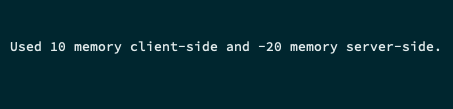
\includegraphics{memUsage.png}
            \caption{A very peculiar memory usage}
            \label{fig:memUsage}
        \end{figure}


\chapter{Evaluation}

    Code validation, analysis of results and practical applications, personal experience

    No coverage/automated tests due to the complexity and erratic nature of the software


\chapter{Conclusions}

    Results wrt objectives, limitations

    Thanks to my advisor, Daniele and everyone that supported me


	\section{Future work and possible developments}

        While this project can be considered a success, there are still a number of improvements
        that could be done. For example a better handling of the data dumping via a separate thread,
        since now every function writes the buffered metrics when it finished executing. While this
        is barely noticeable on a small scale, it could add a significative overhead under large loads.\\

        A crucial missing part is an actual instrumentation like Freud's, either with PIN or another
        library, to allow for direct instrumentation of executables instead of changing the source code.

        Another possible improvement would be to support more complex features, like structs.
